\documentclass[a4paper, 12pt, twoside]{article}


%------------------------------------------------------------------------
%
% Author                :   Lasercata
% Last modification     :   2023.09.13
%
%------------------------------------------------------------------------


%------------------------------------------------------------------------
% This is a LaTeX template, with some useful commands and environments.
%
% Author                :   Lasercata
% Last modification     :   2023.12.18
% Version               :   v6.0.4
%
%------------------------------------------------------------------------


%------ini
\usepackage[utf8]{inputenc}
\usepackage[T1]{fontenc}


%------geometry
\usepackage[textheight=700pt, textwidth=500pt]{geometry}


%------color
\usepackage{xcolor}
\definecolor{ff4500}{HTML}{ff4500}
\definecolor{00f}{HTML}{0000ff}
\definecolor{0ff}{HTML}{00ffff}
\definecolor{656565}{HTML}{656565}

\newcommand{\Emph}{\textcolor{ff4500}}

\newcommand{\strong}[1]{\textcolor{ff4500}{\bf #1}}
\newcommand{\st}{\color{ff4500}\bf}


%------Code highlighting
%---listings
\usepackage{listings}

\definecolor{cbg}{HTML}{272822}
\definecolor{cfg}{HTML}{ececec}
\definecolor{ccomment}{HTML}{686c58}
\definecolor{ckw}{HTML}{f92672}
\definecolor{cstring}{HTML}{e6db72}
\definecolor{cstringlight}{HTML}{98980f}
\definecolor{lightwhite}{HTML}{fafafa}

\lstdefinestyle{DarkCodeStyle}{
    backgroundcolor=\color{cbg},
    commentstyle=\itshape\color{ccomment},
    keywordstyle=\color{ckw},
    numberstyle=\tiny\color{cbg},
    stringstyle=\color{cstring},
    basicstyle=\ttfamily\footnotesize\color{cfg},
    breakatwhitespace=false,
    breaklines=true,
    captionpos=b,
    keepspaces=true,
    numbers=left,
    numbersep=5pt,
    showspaces=false,
    showstringspaces=false,
    showtabs=false,
    tabsize=4,
    xleftmargin=\leftskip
}

\lstdefinestyle{LightCodeStyle}{
    backgroundcolor=\color{lightwhite},
    commentstyle=\itshape\color{ccomment},
    keywordstyle=\color{ckw},
    numberstyle=\tiny\color{cbg},
    stringstyle=\color{cstringlight},
    basicstyle=\ttfamily\footnotesize\color{cbg},
    breakatwhitespace=false,
    breaklines=true,
    captionpos=b,
    keepspaces=true,
    numbers=left,
    numbersep=10pt,
    showspaces=false,
    showstringspaces=false,
    showtabs=false,
    tabsize=4,
    frame=L,
    xleftmargin=\leftskip
}

%\lstset{style=DarkCodeStyle}
\lstset{style=LightCodeStyle}
%Usage : \begin{lstlisting}[language=Caml, xleftmargin=xpt] ... \end{lstlisting}


%---Algorithm
\usepackage[linesnumbered,ruled,vlined]{algorithm2e}
\SetKwInput{KwInput}{Input}
\SetKwInput{KwOutput}{Output}

\SetKwProg{Fn}{Function}{:}{}
\SetKwProg{Proc}{Procedure}{:}{}
\SetKw{KwPrint}{Print}

\newcommand\commfont[1]{\textit{\texttt{\textcolor{656565}{#1}}}}
\SetCommentSty{commfont}
\SetProgSty{texttt}
\SetArgSty{textnormal}
\SetFuncArgSty{textnormal}
%\SetProgArgSty{texttt}

\newenvironment{indalgo}[2][H]{
    \begin{algoBox}
        \begin{algorithm}[#1]
            \caption{#2}
}
{
        \end{algorithm}
    \end{algoBox}
}


%---tcolorbox
\usepackage[many]{tcolorbox}

\DeclareTColorBox{emphBox}{O{black}O{lightwhite}}{
    breakable,
    outer arc=0pt,
    arc=0pt,
    top=0pt,
    toprule=-.5pt,
    right=0pt,
    rightrule=-.5pt,
    bottom=0pt,
    bottomrule=-.5pt,
    colframe=#1,
    colback=#2,
    enlarge left by=10pt,
    width=\linewidth-\leftskip-10pt,
}

\DeclareTColorBox{algoBox}{O{black}O{lightwhite}}{
    breakable,
    arc=0pt,
    top=0pt,
    toprule=-.5pt,
    right=0pt,
    rightrule=-.5pt,
    bottom=0pt,
    bottomrule=-.5pt,
    left=0pt,
    leftrule=-.5pt,
    colframe=#1,
    colback=#2,
    width=\linewidth-\leftskip-10pt,
}


%-------make the table of content clickable
\usepackage{hyperref}
\hypersetup{
    colorlinks,
    citecolor=black,
    filecolor=black,
    linkcolor=black,
    urlcolor=black
}


%------pictures
\usepackage{graphicx}
%\usepackage{wrapfig}

\usepackage{tikz}

\usepackage{float} % For [H] in figure env


%------tabular
%\usepackage{color}
%\usepackage{colortbl}
%\usepackage{multirow}


%------Physics
%---Packages
%\usepackage[version=4]{mhchem} %$\ce{NO4^2-}$

%---Commands
\newcommand{\link}[2]{\mathrm{#1} \! - \! \mathrm{#2}}
\newcommand{\pt}[1]{\cdot 10^{#1}} % Power of ten
\newcommand{\dt}[2][t]{\dfrac{\mathrm d #2}{\mathrm d #1}} % Derivative
\renewcommand{\d}{\mathrm d}

\newcommand{\rot}{\vect{\mathrm{rot}}}
\newcommand{\grad}{\vect{\mathrm{grad}}}
\renewcommand{\div}{\mathrm{div}}
\renewcommand{\j}{\vec\jmath}


%------math
%---Packages
%\usepackage{textcomp}
%\usepackage{amsmath}
\usepackage{amssymb}
\usepackage{mathtools} % For abs
\usepackage{stmaryrd} %for \llbracket and \rrbracket
\usepackage{mathrsfs} %for \mathscr{x} (different from \mathcal{x})
\usepackage{esint} % Better integrals (double, triple, \oiint, ...)

%---Commands
%-Sets
\newcommand{\N}{\mathbb{N}} %set N
\newcommand{\Z}{\mathbb{Z}} %set Z
\newcommand{\Q}{\mathbb{Q}} %set Q
\newcommand{\R}{\mathbb{R}} %set R
\newcommand{\C}{\mathbb{C}} %set C
\newcommand{\U}{\mathbb{U}} %set U
\newcommand{\seg}[2]{\left[ #1\ ;\ #2 \right]}
\newcommand{\nset}[2]{\left\llbracket #1\ ;\ #2 \right\rrbracket}

%-Exponantial / complexs
\newcommand{\e}{\mathrm{e}}
\newcommand{\cj}[1]{\overline{#1}} %overline for the conjugate.

%-Vectors
\newcommand{\vect}{\overrightarrow}
\newcommand{\veco}[3]{\displaystyle \vect{#1}\binom{#2}{#3}} %vector + coord

%-Limits
\newcommand{\lm}[2][{}]{\lim\limits_{\substack{#2 \\ #1}}} %$\lm{x \to a} f$ or $\lm[x < a]{x \to a} f$
\newcommand{\Lm}[3][{}]{\lm[#1]{#2} \left( #3 \right)} %$\Lm{x \to a}{f}$ or $\Lm[x < a]{x \to a}{f}$
\newcommand{\tendsto}[1]{\xrightarrow[#1]{}}

%-Integral
\newcommand{\dint}[4][x]{\displaystyle \int_{#2}^{#3} #4 \mathrm{d} #1} %$\dint{a}{b}{f(x)}$ or $\dint[t]{a}{b}{f(t)}$

%-left right
\newcommand{\lr}[1]{\left( #1 \right)}
\newcommand{\lrb}[1]{\left[ #1 \right]}
\newcommand{\lrbb}[1]{\left\llbracket #1 \right\rrbracket}
\newcommand{\set}[1]{\left\{ #1 \right\}}
\newcommand{\abs}[1]{\left\lvert #1 \right\rvert}
\newcommand{\norm}[1]{\left\lVert #1 \right\rVert}
\newcommand{\ceil}[1]{\left\lceil #1 \right\rceil}
\newcommand{\floor}[1]{\left\lfloor #1 \right\rfloor}
\newcommand{\lrangle}[1]{\left\langle #1 \right\rangle}

%-Boxes
\newcommand{\oboxed}[1]{\textcolor{ff4500}{\boxed{\textcolor{black}{#1}}}} %orange boxed

\newcommand{\rboxed}[1]{\begin{array}{|c} \hline #1 \\ \hline \end{array}} %boxed with right opened
\newcommand{\lboxed}[1]{\begin{array}{c|} \hline #1 \\ \hline \end{array}} %boxed with left opened

\newcommand{\orboxed}[1]{\textcolor{ff4500}{\rboxed{\textcolor{black}{#1}}}} %orange right boxed
\newcommand{\olboxed}[1]{\textcolor{ff4500}{\lboxed{\textcolor{black}{#1}}}} %orange left boxed

%-Others
\newcommand{\para}{/\!/} %//
\newcommand{\ssi}{\ \Leftrightarrow \ }
\newcommand{\eqsys}[2]{\begin{cases} #1 \\ #2 \end{cases}}

\newcommand{\med}[2]{\mathrm{med} \left[ #1\ ;\ #2 \right]}  %$\med{A}{B} -> med[A ; B]$
\newcommand{\Circ}[2]{\mathscr{C}_{#1, #2}}

\renewcommand{\le}{\leqslant}
\renewcommand{\ge}{\geqslant}


%------commands
%---to quote
\newcommand{\simplecit}[1]{\guillemotleft$\;$#1$\;$\guillemotright}
\newcommand{\cit}[1]{\simplecit{\textcolor{656565}{#1}}}
\newcommand{\quo}[1]{\cit{\it #1}}

%---to indent
\newcommand{\ind}[1][20pt]{\advance\leftskip + #1}
\newcommand{\deind}[1][20pt]{\advance\leftskip - #1}

%---to indent a text
\newcommand{\indented}[2][20pt]{\par \ind[#1] #2 \par \deind[#1]}
\newenvironment{indt}[2][20pt]{#2 \par \ind[#1]}{\par \deind} %Titled indented env

%---title
\newcommand{\thetitle}[2]{\begin{center}\textbf{{\LARGE \underline{\Emph{#1} :}} {\Large #2}}\end{center}}

%---Maths environments
%-Proofs
\newenvironment{proof}[1][{}]{\begin{indt}{$\square$ #1}}{$\blacksquare$ \end{indt}}

%-Maths parts (proposition, definition, ...)
\newenvironment{mathpart}[1]{\begin{indt}{\boxed{\text{\textbf{#1}}}}}{\end{indt}}
\newenvironment{mathbox}[1]{\boxed{\text{\textbf{#1}}}\begin{emphBox}}{\end{emphBox}}
\newenvironment{mathul}[1]{\begin{indt}{\underline{\textbf{#1}}}}{\end{indt}}

\newenvironment{theo}{\begin{mathpart}{Théorème}}{\end{mathpart}}
\newenvironment{Theo}{\begin{mathbox}{Théorème}}{\end{mathbox}}

\newenvironment{prop}{\begin{mathpart}{Proposition}}{\end{mathpart}}
\newenvironment{Prop}{\begin{mathbox}{Proposition}}{\end{mathbox}}
\newenvironment{props}{\begin{mathpart}{Propriétés}}{\end{mathpart}}

\newenvironment{defi}{\begin{mathpart}{Définition}}{\end{mathpart}}
\newenvironment{meth}{\begin{mathpart}{Méthode}}{\end{mathpart}}

\newenvironment{Rq}{\begin{mathul}{Remarque :}}{\end{mathul}}
\newenvironment{Rqs}{\begin{mathul}{Remarques :}}{\end{mathul}}

\newenvironment{Ex}{\begin{mathul}{Exemple :}}{\end{mathul}}
\newenvironment{Exs}{\begin{mathul}{Exemples :}}{\end{mathul}}


%------page style
\usepackage{fancyhdr}
\usepackage{lastpage}

\setlength{\headheight}{18pt}
\setlength{\footskip}{50pt}

\pagestyle{fancy}
\fancyhf{}
\fancyhead[LE, RO]{\textit{\textcolor{black}{\today}}}
\fancyhead[RE, LO]{\large{\textsl{\Emph{\texttt{\jobname}}}}}

\fancyfoot[RO, LE]{\textit{\texttt{\textcolor{black}{Page \thepage /}\pageref{LastPage}}}}
% \fancyfoot[LO, RE]{\includegraphics[scale=0.12]{/home/lasercata/Pictures/1.images_profil/logo/mieux/lasercata_logo_fly_fond_blanc.png}}
% \newcommand{\setlogo}{\fancyfoot[LO, RE]{\includegraphics[scale=0.12]{/home/lasercata/Pictures/1.images_profil/logo/mieux/lasercata_logo_fly_fond_blanc.png}}}
\newcommand{\setlogo}[1][/home/lasercata/Pictures/1.images_profil/logo/mieux/lasercata_logo_fly_fond_blanc.png]{\fancyfoot[LO, RE]{\includegraphics[scale=0.12]{#1}}}


%------init lengths
\setlength{\parindent}{0pt} %To avoid using \noindent everywhere.
\setlength{\parskip}{3pt}


\usetikzlibrary{shapes.geometric}
\usetikzlibrary{automata}
\usetikzlibrary{patterns}


%---------------------------------Begin Document
\begin{document}
    
    \thetitle{Tikz}{Testing trees, graphs, ...}
    
    %\tableofcontents
    %\newpage
    
    
%     \begin{indt}{\section{First part :}}
%         
%         .a
%         
%     \end{indt}
    
    \begin{tikzpicture}
        \node [circle, draw] {$\phantom n$}  %[sibling distance = 60pt]
            child {node [circle, draw, xshift=-30pt] {b}
                child {node [circle, draw] {ba}
                    child {node [circle, draw] {bal}}
                }
                child {node [circle, draw] {bo}
                    child {node [circle, draw] {bol}}
                }
            }
            child {node [circle, draw, xshift=30pt] {t}
                child {node [circle, draw, xshift=-20pt] {ta}
                    child {node [circle, draw] {tas}}
                }
                child {node [circle, draw, xshift=20pt] {ti}
                    child {node [circle, draw] {tip}
                        child {node [circle, draw] {tipi}}
                    }
                    child {node [circle, draw] {tir}}
                    child {node [circle, draw] {tic}}
                }
            };
    \end{tikzpicture}
    
    \begin{tikzpicture}
        \node [circle, draw] {$\phantom z$}
            child {node [circle, draw, xshift=-80pt, yshift=20pt] {b}
                child {node [circle, draw, xshift=-50pt, yshift=20pt] {a}
                    child {node [circle, draw, xshift=-25pt, yshift=10pt] {l}
                        child {node [circle, draw, xshift=-20pt] {$\backslash 0$}
                            child {node [circle, draw, xshift=20pt] {l}
                                child {node [circle, draw, xshift=-30pt] {o}
                                    child {node [circle, draw, xshift=-20pt] {n}
                                        child {node [circle, draw, xshift=-10pt] {$\backslash 0$}}
                                    }
                                }
                            }
                        }
                    }
                    child {node [circle, draw, xshift=10pt] {o}
                        child {node [circle, draw, xshift=-20pt] {l}
                            child {node [circle, draw, xshift=-20pt] {$\backslash 0$}}
                        }
                    }
                }
            }
        ;
    \end{tikzpicture}
    
    \newpage
    
    \begin{tikzpicture}
        \node (a) at (0, 0) {$\set{x, y, z}$};
        
        \node (b0) at (-2, -1) {$\set{x, y}$};
        \node (b1) at (0, -1) {$\set{x, z}$};
        \node (b2) at (2, -1) {$\set{y, z}$};
        
        \node (c0) at (-2, -2) {$\set{x}$};
        \node (c1) at (0, -2) {$\set{y}$};
        \node (c2) at (2, -2) {$\set{z}$};
        
        \node (d) at (0, -3) {$\varnothing$};
        
        \draw[->] (d) -- (c0);
        \draw[->] (d) -- (c1);
        \draw[->] (d) -- (c2);
        
        \draw[->] (c0) -- (b0);
        \draw[->] (c0) -- (b1);
        
        \draw[->] (c1) -- (b0);
        \draw[->] (c1) -- (b2);
        
        \draw[->] (c2) -- (b1);
        \draw[->] (c2) -- (b2);
        
        \draw[->] (b0) -- (a);
        \draw[->] (b1) -- (a);
        \draw[->] (b2) -- (a);
    \end{tikzpicture}
    
    
    \begin{tikzpicture}[node distance = 50pt]
        \node (a) at (0, 0) {$\set{x, y, z}$};
        
        \node (b0) [below left of = a] {$\set{x, y}$};
        \node (b1) [below of = a] {$\set{x, z}$};
        \node (b2) [below right of = a] {$\set{y, z}$};
        
        \node (c0) [below of = b0] {$\set{x}$};
        \node (c1) [below of = b1] {$\set{y}$};
        \node (c2) [below of = b2] {$\set{z}$};
        
        \node (d) [below of = c1] {$\varnothing$};
        
        \draw[->] (d) -- (c0);
        \draw[->] (d) -- (c1);
        \draw[->] (d) -- (c2);
        
        \draw[->] (c0) -- (b0);
        \draw[->] (c0) -- (b1);
        
        \draw[->] (c1) -- (b0);
        \draw[->] (c1) -- (b2);
        
        \draw[->] (c2) -- (b1);
        \draw[->] (c2) -- (b2);
        
        \draw[->] (b0) -- (a);
        \draw[->] (b1) -- (a);
        \draw[->] (b2) -- (a);
    \end{tikzpicture}
    
    
    \begin{tikzpicture}[node distance = 50pt, thick]
        \node (e) at (0, 0) {E};
        \node (b) [circle, draw, right of = e] {b};
        \node (c) [rectangle, draw, right of = b] {c};
        \node (s) [below of = b] {S};
        
        \draw[->] (e) -- (b);
        \draw[->] (b) -- node[above] {true} (c);
        \draw[->] (b) -- node[right] {false} (s);
        
        \draw[->] (c) to [out=100, in=80] (b);
    \end{tikzpicture}
    
    \begin{tikzpicture}[node distance = 35pt]
        \node (E) {E};
        \node (I1) [right of = E] {I$_1$};
        \node (X) [right of = I1] {X};
        \node (I2) [right of = X] {I$_2$};
        \node (Y) [right of = I2] {Y};
        \node (S) [right of = Y] {S};
        
        \node (S2) [below right of = I2] {S};
        
        \node (I22) [below of = I1] {I$_2$};
        \node (Y2) [right of = I22] {Y};
        \node (S3) [right of = Y2] {S};
        
        \node (S4) [below right of = I22] {S};
        
        
        \draw[->] (E) -- (I1);
        \draw[->] (I1) -- (X);
        \draw[->] (X) -- (I2);
        \draw[->] (I2) -- (Y);
        \draw[->] (Y) -- (S);
        
        \draw[->] (I2) -- (S2);
        
        \draw[->] (I1) -- (I22);
        \draw[->] (I22) -- (Y2);
        \draw[->] (Y2) -- (S3);
        
        \draw[->] (I22) -- (S4);
    \end{tikzpicture}
    
    \vspace{12pt}
    
    \begin{tikzpicture}
        \draw(2, 0) rectangle (4,1);
        \draw[-](3,0)--(3,1);
        \draw [-stealth, thick] (3.4, 0.5)--(5, 0.5);
        \draw(5, 0) rectangle (6,1);
        \draw(6, 0) rectangle (7,1);
        \draw [-stealth, thick] (6.4, 0.5)--(8, 0.5);
        \draw(8, 0) rectangle (9,1);
        \draw(9, 0) rectangle (10,1);
        
        \foreach \pos in {(2.5,1.255),(5.5, 1.255),(8.5, 1.255)}
            \node at \pos {elem};        
        \foreach \pos in {(3.5, 1.25),(6.5, 1.25)}
            \node at \pos {next};
        \node at (9.5, 0.5) {NULL};
    \end{tikzpicture}
    
    \begin{tikzpicture}
        \draw(2, 0) rectangle (4, 1);
        \draw[-] (3, 0) -- (3, 1);
        \draw [->] (3.4, 0.5)--(5, 0.5);
    \end{tikzpicture}
    
    \begin{tikzpicture}
        \draw[step=1cm] (0, 0) grid (4, 4);
        \draw[fill] (.5, .5) circle (.25cm);
    \end{tikzpicture}
    
    \begin{tikzpicture}[xslant=-1, yslant=-.1]
        \draw[step=1cm] (0, 0) grid (4, 4);
        \draw[fill] (.5, .5) circle (.25cm);
    \end{tikzpicture}
    
    \begin{tikzpicture}[yshift=-83,every node/.append style={yslant=0.5, xslant=-1}, yslant=0.5, xslant=-1]
        \draw[step=1cm] (0, 0) grid (4, 4);
        \draw[fill] (.5, .5) circle (.25cm);
    \end{tikzpicture}
    
    
    \begin{tikzpicture}[border/.style={fill=gray!50, ultra thick}]
        \def\n{5}
        \foreach \i/\j in {0/0, 0/3, 3/0, 2/3}
            \draw[border] (\i, \j) rectangle (\i + 2, \j + 2);
        \draw[border] (1, 3) --++ (2, 0) --++ (0, -2) --++ (-1, 0) --++ (0, 1) --++ (-1, 0) -- cycle;
        \draw[border] (3, 2) --++ (2, 0) --++ (0, 2) --++ (-1, 0) --++ (0, -1) --++ (-1, 0) -- cycle;
        \foreach \i in {0, ..., \n} {
            \draw (\i, 0) -- (\i, \n);
            \draw (0, \i) -- (\n, \i);
        }
    \end{tikzpicture}
    
    
    \begin{center}
        \begin{tikzpicture}[terme/.style={shape=rectangle, rounded corners=3pt, draw=ff4500}, atome/.style={shape=circle, draw=blue}]
            \node {$\wedge$}
                child {node [xshift=-20pt] {$\forall A$}
                    child {node {$\forall B$}
                        child {node {$\subseteq$}
                            child {node (cap) {$\cap$}
                                child {node {$A$}}
                                child {node {$B$}}
                            }
                            child {node (A)  [terme] {$A$}}
                        }
                    }
                }
                child {node [xshift=20pt] {$\subseteq$}
                    child {node (v)  [terme] {$\varnothing$}}
                    child {node [terme] {$A$}}
                }
            ;
            
            \draw[terme] (-3.2, -7.8) rectangle (-1.2, -5.75);
            \draw[atome] (-1.5, -6.5) circle (2.3cm);
            \draw[atome] (1.47, -2.5) circle (1.35cm);
            
            \matrix [draw, below left, rounded corners=5pt] at (5, -5) {
                \node [terme, label=right:terme] {}; \\
                \node [atome, label=right:atome] {}; \\
            };
        \end{tikzpicture}
    \end{center}
    
    
    \begin{center}
        \begin{tikzpicture}
            %\draw (0, 0) circle (2);
            
            \draw plot [smooth cycle, tension=.7] coordinates {(0:2.5) (30:2.7) (60:2) (90:2.5) (120:2.3) (150:1.8) (180:2) (210:2) (240:2) (270:2.3) (300:2.5) (330:2.5)};

            \node (B) at (120:1.5) {$B$};
            
            \draw [dashed] plot [smooth, tension=1] coordinates {(-5:2.5) (-10:1) (-50:2.5) (-65:3.5) (-90:2.3)};
            
            %\node (0) at (0, 0) {$+$};
            
            \node [label=right:$s_i$] (s) at (-20:1.6) {$+$};
            
            \node [label=left:$v$] (v) at (-62:3) {$+$};
            
            \draw[->] (s) -- (v);
            \draw[->] (s) -- (0, 0);
            \draw[->] (s) -- (1, 1);
        \end{tikzpicture}
    \end{center}
    
    \begin{tikzpicture}
        \draw[rounded corners=5pt] (0, 0) rectangle (1, 2);
    \end{tikzpicture}
    

    \begin{center}
        \begin{tikzpicture}[scale=2]
            \foreach \i in {0, 1, 2} {
                \foreach \j in {0, 1, 2} {
                    \node (\i\j) at (\i, \j) [circle, draw] {\i\j};
                }
            }

            \draw (00) -- (10);
            \draw (00) -- (01);
            \draw (00) -- (11);
        \end{tikzpicture}
    \end{center}

    \begin{center}
        \begin{tikzpicture}
            \foreach \i in {0, 1, ..., 4} {
                \node (\i) at (\i*72:1) [circle, draw] {};
            }

            \foreach \i in {0, 1, ..., 4} {
                \foreach \j in {0, 1, ..., 4} {
                    \draw[color=ff4500] (\i) -- (\j);
                }
            }

            \draw (0) -- (1) -- (2) -- (3) -- (4) -- (0);
        \end{tikzpicture}
    \end{center}
    
    \begin{center}
        \begin{tikzpicture}[scale=1.4]
            \foreach \i in {0, 1, ..., 4} {
                \node (\i) at (\i*72+90 : 1) [circle, draw] {\i};
                \draw (\i*72+90+36 : .5) to (\i*72+90+36 : 1.5);      
            }

            \foreach \i in {1, 2, 3, 4} {
                \draw[dashed] (\i) -- (\i*72+90+36 : 1);
            }

            %\node at (0, 0) {$\cdot$};
        \end{tikzpicture}
    \end{center}
    
    \begin{center}
        \begin{tikzpicture}
            \node (t) at (-1, 0) {$t$};

            \foreach \i in {0, 1, 2, 3} {
                \node (s\i) at (3*\i, 0) {\tiny{$\blacksquare$}};
                \draw (3*\i, 0) rectangle (3*\i+2, 1);
                \draw (3*\i+1, 0) -- (3*\i+1, 1);
                \ifnum \pdfstrcmp{\i}{3}=0
                    \node (b\i) at (3*\i+1.5, .5) {\Huge{$\times$}};
                \else
                    \node (b\i) at (3*\i+1.5, .5) {$\bullet$};
                \fi
            }

            \node at (.5, .5) {$-\infty$};
            \node at (3.5, .5) {$3$};
            \node at (6.5, .5) {$8$};
            \node at (9.5, .5) {$+\infty$};

            \foreach \i/\j in {0/1, 1/2, 2/3} {
                \draw[->] (b\i) to (s\j);
            }

            \draw[->] (t) to (s0);
        \end{tikzpicture}
    \end{center}
    
    \begin{center}
        \begin{tikzpicture}[scale=1.5]
            \node (0) at (0, 0) [state] {$q_0$};
            \node (LPAR) at (40: 3) [state] {$q_{\rm LPAR}$};
            \node (RPAR) at (0: 3) [state] {$q_{\rm RPAR}$};
            \node (DOT) at (320: 3) [state] {$q_{\rm DOT}$};
            \node (l) at (280: 3) [state] {$q_l$};
            \node (LBD) at (200: 3) [state] {$q_{\rm LBD}$};
            \node (lb) at (240: 3) [state] {$q_{\rm lb}$};
            \node (x) at (160: 3) [state] {$q_x$};
            \node (VAR) at (120: 3) [state] {$q_{\rm VAR}$};
            \node (EOF) at (80: 3) [state, accepting] {$q_{\rm EOF}$};

            %Initial arrow for the initial state.
            \draw[->] (240: .9) to (0);

            \draw[->] (0) to [out=50, in=-150] node [above left] {\small{$($}} (LPAR);
            \draw[->] (LPAR) to [out=-130, in=30] node [below, rotate=40] {\tiny{OUT: LPAR}} (0);

            \draw[->] (0) to [out=10, in=170] node [above] {\small{$)$}} (RPAR);
            \draw[->] (RPAR) to [out=-170, in=-10] node [below] {\tiny{OUT: RPAR}} (0);

            \draw[->] (0) to [out=-30, in=130] node [above right] {$\cdot$} (DOT);
            \draw[->] (DOT) to [out=150, in=-50] node [below, rotate=-40] {\tiny{OUT: DOT}} (0);

            \draw[->] (0) to node [right] {$l$} (l);
            \draw[->] (l) to node [below right] {$b$} (lb);
            \draw[->] (lb) to node [below left] {$d$} (LBD);
            \draw[->] (LBD) to node [above, rotate=20] {\tiny{OUT: LAMBDA}} (0);

            \draw[->] (0) to node [above right] {$x$} (x);
            \draw[->] (x) to node [above left] {$0 - 9$} (VAR);
            \draw[->] (VAR) to node [below, rotate=-60] {\tiny{OUT: VAR}} (0);

            \draw[->] (0) to node [above, rotate=80] {\tiny{OUT: EOF}} (EOF);
        \end{tikzpicture}
    \end{center}
    
    
    \begin{center}
        \begin{tikzpicture}
            \draw[rounded corners=5pt] (0, 0) to (1, 0) to (1, 1);
            
            \draw (2, 0) to (3, 0) to [out=0, in=-90] (3.5, .5) to (3.5, 1);
        \end{tikzpicture}
    \end{center}
    
    \begin{center}
        \begin{tikzpicture}
            \node (0) at (0, 0) {$\bullet$}
                child [xshift=-90pt] {node {$\bullet$}
                    child [xshift=-30pt] {node {$\bullet$}
                        child {node {} edge from parent [dashed]}
                        edge from parent [above left] node {$x_2 = 1$}
                    }
                    child [xshift=30pt] {node {$\bullet$}
                        child {node {$\bullet$}
                            child {node {} edge from parent [dashed]}
                            edge from parent [above left] node {$x_3 = 1$}
                        }
                        child {node {$\bullet$}
                            child {node {} edge from parent [dashed]}
                            edge from parent [above right] node {$x_3 = 0$}
                        }
                        edge from parent [above right] node {$x_2 = 0$}
                    }
                    edge from parent [above left] node {$x_1 = 1$}
                }
                child [xshift=90pt] {node {$\bullet$}
                    child [xshift=-30pt] {node {$\bullet$}
                        child {node {$\bullet$}
                            child {node {} edge from parent [dashed]}
                            edge from parent [above left] node {$x_3 = 1$}
                        }
                        child {node {$\bullet$}
                            child {node {} edge from parent [dashed]}
                            edge from parent [above right] node {$x_3 = 0$}
                        }
                        edge from parent [above left] node {$x_2 = 1$}
                    }
                    child [xshift=30pt] {node {$\bullet$}
                        child {node {$\bullet$}
                            child {node {} edge from parent [dashed]}
                            edge from parent [above left] node {$x_3 = 1$}
                        }
                        child {node {$\bullet$}
                            child {node {} edge from parent [dashed]}
                            edge from parent [above right] node {$x_3 = 0$}
                        }
                        edge from parent [above right] node {$x_2 = 0$}
                    }
                    edge from parent [above right] node {$x_1 = 0$}
                }
            ;

            \node (1) at (-6, -6) {
                \begin{tabular}{c}
                    Sous-arbre non parcouru
                    \\
                    car dépasse la capacité
                \end{tabular}
            };
            \draw[->] (1) to (-5.7, -4.5);
        \end{tikzpicture}
    \end{center}

    \begin{center}
        \begin{tikzpicture}[domain=0:5]
            \draw[->] (0, 0) to (6, 0);
            \draw[->] (0, 0) to (0, 6);
            
            \draw [color=ff4500] plot (\x, {-.8 * (\x - 1) * (\x - 4) + 3.2});

            %\node (1) at (0, 0) {$\times$};
            %\node (2) at (.5, 1.8) {$\times$};
            %\node (3) at (1, 3.2) {$\times$};
            %\node (4) at (1.5, 4.2) {$\times$};
            %\node (5) at (2.5, 5) {$\times$};
            %\node (6) at (3.5, 4.2) {$\times$};
            %\node (7) at (4, 3.2) {$\times$};
            %\node (8) at (4.5, 1.8) {$\times$};
            %\node (9) at (5, 0) {$\times$};

            \node (1) at (0, 0) {$\times$};
            \node (2) at (.4, 2.1) {$\times$};
            \node (3) at (1, 2.8) {$\times$};
            \node (4) at (1.5, 4.2) {$\times$};
            \node (5) at (2.5, 5.5) {$\times$};
            \node (6) at (3.4, 4.0) {$\times$};
            \node (7) at (4.2, 3.3) {$\times$};
            \node (8) at (4.4, 1.8) {$\times$};
            \node (9) at (5, 0) {$\times$};

            %\draw [color=blue] plot [smooth] coordinates {(1) (2) (.6, 1.8) (3) (1.20, 4.1) (4) (2, 4.3) (5) (2.9, 5.5) (6) (7) (4.25, 2.2) (8) (9)};
            \draw [color=blue] plot [smooth] coordinates {(1) (2) (3) (4) (5) (6) (7) (8) (9)};
        \end{tikzpicture}
    \end{center}
 
    
    \begin{center}
        \begin{tikzpicture}
            \draw[->] (0, 0) to (5, 0);
            \draw[->] (0, 0) to (0, 5);

            \draw (0, 0) to (4.5, 4.5);

            \node at (3, 2) [color=red] {$\times$};

            \node (1) at (.25, 1.5) {$\times$};
            \node (2) at (.6, 2.8) {$\times$};
            \node (3) at (1.2, 3.9) {$\times$};
            \node (4) at (2.3, 4.3) {$\times$};
            \node (5) at (3.5, 4.45) {$\times$};

            \draw[color=ff4500] plot [smooth, tension=.6] coordinates {(0, 0) (1) (2) (3) (4) (5) (4.5, 4.5)};

            \fill [pattern = dots] % needs \usetikzlibrary{patterns}
                (0, 0)
                -- plot [smooth, tension=.6] coordinates {(0, 0) (1) (2) (3) (4) (5) (4.5, 4.5)}
                -- (4.5, 4.5);
        \end{tikzpicture}
    \end{center}
    
    \begin{center}
        \begin{tikzpicture}
            \draw[->] (0, 0) to (5, 0);
            \draw[->] (0, 0) to (0, 5);

            \draw (0, 0) to (4.5, 4.5);

            \node at (3, 2) [color=red] {$\times$};

            \node (1) at (.25, 1.5) {$\times$};
            \node (2) at (.6, 2.8) {$\times$};
            \node (3) at (1.2, 3.9) {$\times$};
            \node (4) at (2.3, 4.3) {$\times$};
            \node (5) at (3.5, 4.45) {$\times$};

            \draw[color=ff4500] plot [smooth, tension=.6] coordinates {(0, 0) (1) (2) (3) (4) (5) (4.5, 4.5)};

            \fill [pattern = north west lines] % needs \usetikzlibrary{patterns}
                (0, 0)
                -- plot [smooth, tension=.6] coordinates {(0, 0) (1) (2) (3) (4) (5) (4.5, 4.5)}
                -- (4.5, 4.5);
        \end{tikzpicture}
    \end{center}


    \begin{center}
        \begin{tikzpicture}
            \draw[->] (-.5, 0) to (9, 0);
            \draw[->] (0, -3) to (0, 3);

            \node (x) at (9.3, -.3) {$x$};
            \node (y) at (0.3, 3.3) {$y$};

            \draw [domain=0:2.6 * 3.141, smooth, blue] plot (\x, {2*cos(\x * 180 / 3.14)});
            \draw [dashed, domain=0:2.6 * 3.141, smooth, blue] plot (\x, {-2*cos(\x * 180 / 3.14)});
            \draw [domain=0:2.5 * 3.141, ff4500, samples=250] plot (\x, {2*cos(\x * 180 / 3.14) * cos(10 * \x * 180 / 3.14)});
        \end{tikzpicture}
    \end{center}


    \begin{center}
        \begin{tikzpicture}
            \draw[->] (-.5, 0) to (12, 0);
            \draw[->] (0, -3) to (0, 3);

            \node (x) at (12.3, -.3) {$x$};
            \node (y) at (0.3, 3.3) {$y$};

            \draw [domain=0:2.1 * 3.141, smooth, blue] plot (\x, {2*cos(\x * 180 / 3.14)});
            \draw [domain=0:2 * 3.141, smooth, ff4500] plot (\x, {cos(\x * 180 / 3.14)});

            \draw [dashed] (2 * 3.141, 0) -- (2 * 3.141, 2);
            \node at (6.281, -.5) {$\dfrac{2\pi}{k}$};

            \node (A) at (0, 2) [label=left:{$2A_0$}] {$-$};
            \node (A-) at (0, -2) [label=left:{$-2A_0$}] {$-$};
        \end{tikzpicture}
    \end{center}

    
\end{document}
%--------------------------------------------End
